%!TEX root = ../report.tex

% 
% Architecture
% 

\section{Solution's Architecture Proposal}

Considering this project problem and the objectives presented in problem contextualization section, We want to develop a process framework for project and maintenance management to be applied to an Information Systems administration. We provided, in Related Work section, a state of the art ins several frameworks for IT governance and management, as well as international standards, building a knowledge base to start planning and designing the processes.\par
Taking in account the complexity of some frameworks presented, like COBIT, and also the problem's scope and the solution time-frame, we need to conduct an analysis of the knowledge we will use from each framework or standard. We will use ISO/IEC 12207, presented in section 5.1, to define which types of processes we will consider for this project, defining next the frameworks and standards we will consider as reference for each type of processes. As long as processes need supporting artifacts and a responsibility structure, this references also support this needs, presenting some suggestions of how responsibilities are addressed for each process and what artifacts are needed for a correct process implementation.\par
Since we are also looking for a logical application architecture, we will provide a deeper analysis on the solutions present in section 6, narrowing down the available solutions to provide the features more important for this project, in order to reach to an logical application architecture that is able to fully support our process framework.\par
As long as this project is aligned with a real-case scenario for an organization, we will take design decisions considering the stakeholders for this project, specially when dealing with the choice of the type of processes to consider and the solutions choosing for integrating the logical application architecture. This organization will also provide us ways to demonstrate our solution's suitability, allowing us to achieve the demonstration and evaluation step of the DSRM process applied for this project\par



\subsection{Process Framework}

To start designing our processes, we need first to define what processes we will consider to be in the scope of this project. For this, and taking as reference ISO/IEC 12207, detailed in section 5.1, that standardizes the processes for the whole life cycle of software, we will present the areas we will address and the reasons why we do not do it for the others.\par
The two main areas to consider are governance and management processes. Considering the extensibility and complexity of both, we could not focus on the two giving the time-frame available. Being so, we decided, accordingly with the stakeholders, to not detail governance processes. Areas focused on organization strategy or project portfolio will not be addressed for this project. Instead, we will consider that this subjects are already clearly defined by the organization, being our responsibility designing processes that comply with them. 
Despite this, there are governance processes that will have direct influence on the subjects covered by this thesis, namely risk, budget and quality management. These subjects will be addressed by this project considering a more operational approach. We will consider that organization strategy for this areas is already defined, being our mission design processes that implement and ensure this strategy in practice.\par



\subsubsection{Processes definition}


The areas of interest were chosen based on stakeholders' needs for this project. As long as it is aligned with a real-case organization, we had to proceed to interviews with stakeholders as a way to define the problem, namely the areas of interest we need to cover. This areas were chosen in agreement with the two parties involved in this project, bu it can be changed during project execution.\par
Our idea with this project is to provide a more general process framework for project and maintenance management, but that would be applicable to this organization particular scenario. Based on this, the processes we will consider are aligned with this objective, being, in our shared opinion, the most important to consider in this scenario. Also, more areas can be covered in the future, if we consider it is a added value for this framework.  
In figure 32 we can observe the areas of interest for this project highlighted from the ISO/IEC 12207 international standard reference for software life cycle processes. This standard was considered because we needed a starting point to define the processes scope for this project. Groups of processes directly related to governance are not considered for this project, as the Agreement processes and Organizational Project-Enabling processes.\par
Technical Processes and Software Implementation processes are also not considered in the scope, because we will assume that projects implementation is outsourced, being responsibility of a third-party. In light of this, processes presented in Technical and Software Implementation processes groups are not relevant for the organization, although  they are fundamental for the third-party that will implement the project. Despite this assumption, the organization itself has a complete process for project management, that is different from the third-party project. Aspects like project calendar, deliveries and control are done by the two entities by different perspectives, being us responsible for the organization project management.\par
For this thesis, we will consider the Project processes and the Software Support processes, both directly related to project and maintenance management. In addition to the processes in Project processes group, we will also consider Capacity Management, Issues Management,Financial Management and Document Management as processes belonging to this group.\par
Regarding Software Support Processes, we will consider Software Documentation Management, Software Configuration Management and Software Validation and audit processes.\par
Software Reuse Processes group will not be considered for this project because are not considered as a theme of interest for it, being also not related with the objectives we purpose. In next section we will present how we will address each one of the processes, considering the available state of the art.\par

\begin{figure}[h!]
\centering
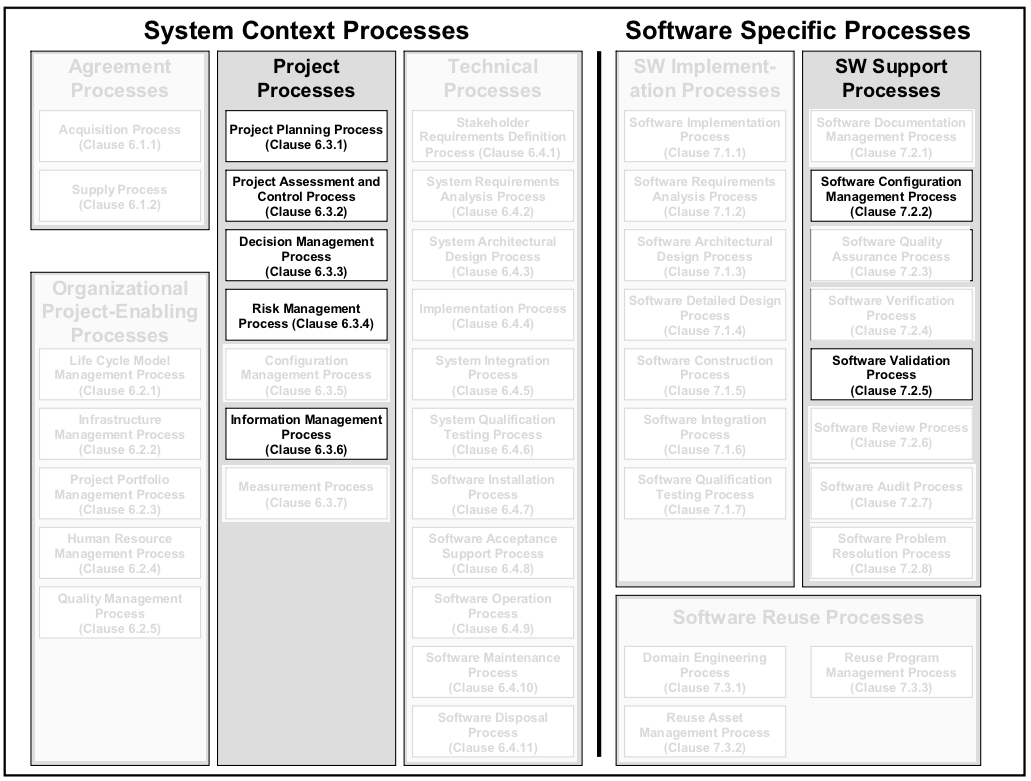
\includegraphics[width=0.8\textwidth]{img/ISO12207ProcessesImplemented.png}
\caption{Processes areas considered for this project. Adapted from \cite{ISO12207}.}
\end{figure}

Capacity Management, issues Management, Financial Management and Document Management are process areas that are not clearly addressed by ISO/IEC 12207, but were processes necessary to consider based on stakeholders needs.\par
Capacity Management, as stated in \cite{itilSD}, ``ensure that cost-justifiable IT capacity in all areas of IT always exists and is matched to the current and future agreed needs of the business, in a timely manner.''. It is point were all performance and capacity subjects are dealt, considering resources and services itself. Capacity management is focused on two operations: balancing costs against resources needed and balancing supply against demand.\par
Capacity Management is divided in three main areas: Business Capacity Management (business needs and plans translation into requirements for service and IT infrastructure), Service Capacity Management (management, control and prediction of performance and capacity of IT services operation) and Component Capacity Management (management, control and prediction of the performance, utilization and capacity of individual IT technology components).\par
Issues Management is the process of identifying and resolving issues, as staff, supplier, technical or material problems. Many times confused with risks, issues have a more unpredictable profile. They can arise from project processes with no warning or no expectation at all. Usually risks are more predictable are are known on project start. Most organizations find difficult to manage issues from an effectively manner and many times it a process that is not implemented across the complete organization, making more difficult issues resolution.\par
As stated in \cite{itilSS}, ``Financial Management provides the business and IT with the quantification, in financial terms, of the value of IT Services, the value of the assets underlying the provisioning of those services, and the qualification of operational forecasting''. As the main areas for IT Financial Management we have Budgeting (Expenditures planning and controlling), IT accounting (Cost analysis on IT services providing) and Charging (Costs assignment to IT services provided). Financial Management is a complex area and we need a more deeper analysis on this processes importance for our processes framework, in order to only provide the needed financial activities for reducing complexity.\par
Documentation Management corresponds to an area that deals with all documentation concerns on an organization, from technical documentation to project management documentation. This area groups processes for plan, production, tracking and communication of documents produced by the organization in project and maintenance contexts. This processes are also related to the supporting artifacts we want to develop for our process framework and need to be taken in account to achieve successful for the whole processes.\par
In table 2 is presented a table with the processes group we will consider for this project and a description of some activities each process intents to implement.

\begin{table}[h!]
\centering
\resizebox{\textwidth}{!}{%
\begin{tabular}{|l|c|c|c|c|c|c|c|c|c|c|c|c|c|}
\hline
\multicolumn{1}{|c|}{} & \multicolumn{4}{c|}{\textbf{COBIT 5 Domains}} & \multicolumn{5}{c|}{\textbf{ITIL V3 Volumes}} &  &  &  &  \\ \cline{2-10}
\multicolumn{1}{|c|}{\multirow{-2}{*}{\textbf{Processes}}} & \textbf{APO} & \textbf{BAI} & \textbf{DSS} & \textbf{MEA} & \textbf{SS} & \textbf{SD} & \textbf{SO} & \textbf{ST} & \textbf{CSI} & \multirow{-2}{*}{\textbf{PMBOK}} & \multirow{-2}{*}{\textbf{\begin{tabular}[c]{@{}c@{}}ISO/IEC\\ 20000\end{tabular}}} & \multirow{-2}{*}{\textbf{\begin{tabular}[c]{@{}c@{}}ISO/IEC \\ 27000\end{tabular}}} & \multirow{-2}{*}{\textbf{\begin{tabular}[c]{@{}c@{}}ISO\\ 31000\end{tabular}}} \\ \hline
\textbf{Project Planning} & \cellcolor[HTML]{5A9D58}\checkmark & \cellcolor[HTML]{5A9D58}\checkmark &  &  &  &  &  &  &  & \cellcolor[HTML]{FD6864}\checkmark & \cellcolor[HTML]{329A9D}\checkmark &  &  \\ \hline
\textbf{Project Assessment and Control} & \cellcolor[HTML]{5A9D58}{\color[HTML]{000000} \checkmark} & \cellcolor[HTML]{5A9D58}{\color[HTML]{000000} \checkmark} & \cellcolor[HTML]{5A9D58}{\color[HTML]{000000} \checkmark} & \cellcolor[HTML]{5A9D58}{\color[HTML]{000000} \checkmark} &  &  &  &  &  & \cellcolor[HTML]{FD6864}\checkmark & \cellcolor[HTML]{329A9D}\checkmark &  &  \\ \hline
\textbf{Decision Management} & \cellcolor[HTML]{5A9D58}{\color[HTML]{000000} \checkmark} & \cellcolor[HTML]{5A9D58}{\color[HTML]{000000} \checkmark} & \cellcolor[HTML]{5A9D58}{\color[HTML]{000000} \checkmark} & \cellcolor[HTML]{5A9D58}{\color[HTML]{000000} \checkmark} & \cellcolor[HTML]{FFCC67}\checkmark &  &  &  &  & \cellcolor[HTML]{FD6864}\checkmark & \cellcolor[HTML]{329A9D}\checkmark &  &  \\ \hline
\textbf{Risk Management} & \cellcolor[HTML]{5A9D58}\checkmark &  &  &  &  & \cellcolor[HTML]{FFCC67}\checkmark &  &  &  & \cellcolor[HTML]{FD6864}\checkmark &  & \cellcolor[HTML]{329A9D}\checkmark & \cellcolor[HTML]{329A9D}\checkmark \\ \hline
\textbf{Capacity Management} & \cellcolor[HTML]{5A9D58}\checkmark & \cellcolor[HTML]{5A9D58}\checkmark &  &  &  & \cellcolor[HTML]{FFCC67}\checkmark &  &  &  &  &  &  &  \\ \hline
\textbf{Issues Management} &  &  & \cellcolor[HTML]{5A9D58}\checkmark &  &  &  & \cellcolor[HTML]{FFCC67}\checkmark &  &  &  &  &  &  \\ \hline
\textbf{Financial Management} & \cellcolor[HTML]{5A9D58}\checkmark &  &  &  & \cellcolor[HTML]{FFCC67}\checkmark &  &  &  &  &  &  &  &  \\ \hline
\textbf{Documentation Management} & \cellcolor[HTML]{5A9D58}\checkmark & \cellcolor[HTML]{5A9D58}\checkmark &  &  &  &  &  &  &  & \cellcolor[HTML]{FD6864}\checkmark &  & \cellcolor[HTML]{329A9D}\checkmark &  \\ \hline
\textbf{Software Configuration Management} &  & \cellcolor[HTML]{5A9D58}\checkmark &  &  &  &  &  & \cellcolor[HTML]{FFCC67}\checkmark &  &  &  &  &  \\ \hline
\textbf{Software Validation} & \cellcolor[HTML]{5A9D58}\checkmark &  &  &  &  &  &  & \cellcolor[HTML]{FFCC67}\checkmark &  & \cellcolor[HTML]{FD6864}\checkmark &  &  &  \\ \hline
\end{tabular}
}
\caption{Processes areas and main activities}
\label{my-label}
\end{table}


\subsubsection{Processes Mapping to frameworks}

In this section we will present how each one of the processes in the scope for this project are addressed and mapped into the frameworks and standards presented in section 4 and 5. This will provide us an initial guidance on how we should approach the problem, based on already stated knowledge by professional in the area. Our objective is to use only the important aspects for this project, reducing the complexity of implementing a complete framework for the organization. Consider this, we need to map the processes in the scope for this project to, during processes design, discover what objectives are already covered by the frameworks and which ones need more original work.\par
In table 3 we present the mapping between each processes group in the scope for this project with the framework or standard that covers some aspects for it:\par

\begin{table}[h!]
\centering
\resizebox{0.9\textwidth}{!}{%
\begin{tabular}{|c|l|}
\hline
\textbf{Processes} & \multicolumn{1}{c|}{\textbf{Description}} \\ \hline
\textbf{Project Planning} & \begin{tabular}[c]{@{}l@{}}Scope and goals definition;\\ Requirements establishment;\\ Activities and deliverables identification;\\ Schedule definition;\\ Resources identification;\\ Responsibilities assignment;\\ Quality, Risk and Cost Analysis;\end{tabular} \\ \hline
\textbf{Project Assessment and Control} & \begin{tabular}[c]{@{}l@{}}Project monitoring;\\ Project control;\\ Project assessment;\end{tabular} \\ \hline
\textbf{Decision Management} & \begin{tabular}[c]{@{}l@{}}Decision-Making strategy definition;\\ Alternative Courses of action definition;\\ Course of action identification;\\ Decision analysis;\\ Decision tracking;\end{tabular} \\ \hline
\textbf{Risk Management} & \begin{tabular}[c]{@{}l@{}}Risk Management planning;\\ Risk Profile Management;\\ Risk Analysis;\\ Risk Treatment;\\ Risk Monitoring;\\ Risk Management process evaluation;\end{tabular} \\ \hline
\textbf{Capacity Management} & \begin{tabular}[c]{@{}l@{}}Capacity Plan definition;\\ Performance Monitoring;\\ Performance Analysis;\\ Performance tuning;\end{tabular} \\ \hline
\textbf{Issues Management} & \begin{tabular}[c]{@{}l@{}}Issue Identification;\\ Issue Prioritization;\\ Issue Resolution;\\ Issue Communication;\end{tabular} \\ \hline
\textbf{Financial Management} & \begin{tabular}[c]{@{}l@{}}Budgeting definition;\\ IT Accounting planning;\\ Charging planning;\\ Financial control;\\ Financial communication;\end{tabular} \\ \hline
\textbf{Documentation Management} & \begin{tabular}[c]{@{}l@{}}Documentation definition;\\ Documentation production;\\ Documentation validation;\\ Documentation communication;\\ Documentation tracking;\end{tabular} \\ \hline
\textbf{Software Configuration Management} & \begin{tabular}[c]{@{}l@{}}Software configuration management plan developing;\\ Configuration Identification;\\ Configuration Control;\\ Configuration Status Accounting;\\ Configuration Evaluation;\end{tabular} \\ \hline
\textbf{Software Validation} & \begin{tabular}[c]{@{}l@{}}Validation plan definition;\\ Test requirements, test cases and test specifications preparation;\\ Tests Execution;\\ Software validation against the requirements execution;\end{tabular} \\ \hline
\end{tabular}
}
\caption{Processes Mapping to frameworks and standards}
\label{my-label}
\end{table}

\subsubsection{Processes Supporting artifacts}

Considering the processes framework we want to develop, we need some artifacts to support this processes, namely communication and decisions artifacts that will allow us to support the inputs and outputs for activities in each process. For this, we will provide, in conjunction with the processes framework, all artifacts needed to support it, from templates to decision documents templates, clearly defining its purpose, content and participants.\par
This artifacts will be defined during the designing of the process framework. The frameworks and standards previously presented define some supporting artifacts needed for its processes, considering the inputs and outputs for this processes. Our work will be address the ones we also need for our processes and define new artifacts that not covered by any of the frameworks and standards.\par

\subsubsection{Responsibility Structure}

The developed framework needs to have an inherent responsibility structure, defining the processes' participants and accounted for decisions and activities. This structure is particularly important when considering we are dealing with a real-case organization, that has already an organizational structure defined and for the one we are designing our processes.\par
For designing this responsibility structure we will consider the work already done for the frameworks and standards presented previous in responsibility assignment. COBIT and ITIL present clearly the responsibility structure for its processes. Despite that, we need also to have some original work on this subject, considering we are not implementing directly any of those frameworks. This work will be accomplished during the processes design and taking in account the common responsibility structures on IT organizations.\par 

\subsection{Logical Application Architecture}

\subsubsection{PPM Tools}

\subsubsection{ITSM Tools}

\subsection{Demonstration Proposal}


